\title{Study Guide for Midterm 1 for Algebra-Based Physics-2: Electricity, Magnetism, and Modern Physics (PHYS135B-01)}
\author{Dr. Jordan Hanson - Whittier College Dept. of Physics and Astronomy}
\date{\today}
\documentclass[10pt]{article}
\usepackage[a4paper, total={18cm, 27cm}]{geometry}
\usepackage{outlines}
\usepackage[sfdefault]{FiraSans}
\usepackage{hyperref}
\usepackage{graphicx}
\begin{document}
\maketitle

\begin{enumerate}
\item \textbf{Applications of circuits, Chapter 21}:
\begin{enumerate}
\item A 1000 W toaster and a 1000 W microwave are connected to the 120 V outlet.  Will this blow the 15 A fuse?
\item What is the total resistance of the system?  What is the resistance of each device?
\item If the toaster were disconnected, what would be the total current?
\item What is highest wattage that could be connected to the wall with the microwave that would not blow the 15 A fuse? \\ \vspace{3cm}
\end{enumerate}
\item \textbf{Magnetism, Chapter 22}:
\begin{enumerate}
\item Draw the magnetic field of the Earth, and mark the location of the magnetic south and north poles on the Earth.  Estimate the angle of the Earth's magnetic field with respect to the ground in California, and at the South Pole. \\ \vspace{3cm}
\item What are the signs of the charged particles in Fig \ref{fig:magfield}?
\begin{figure}[ht]
\centering
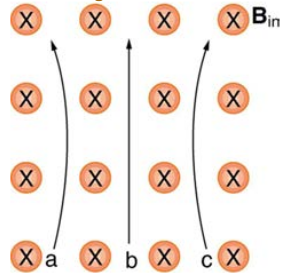
\includegraphics[width=0.2\textwidth]{magfield.png}
\caption{\label{fig:magfield} A magnetic field into the page with three potentially charged particles passing through it.}
\end{figure}
\item If the B-field in Fig. \ref{fig:magfield} has a strength of 0.001 T, and the particles at left and right are moving in circular paths with radius 1.0 m, what is the speed of these particles?
\end{enumerate} \vspace{2cm}
\item \textbf{Magnetism 2, Chapter 23}:
\begin{enumerate}
\item Recall that the definition of magnetic flux through an area $A$ by a B-field $B$ is $\phi = \vec{B} \cdot \vec{A} = BA\cos\theta$. See Fig. \ref{fig:magfield2}.  What is the flux of a 0.001 T B-field passing through an area of 10 cm$^2$ at a 45 degree angle?
\begin{figure}[hb]
\centering
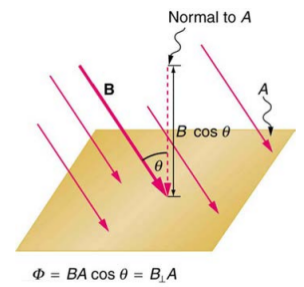
\includegraphics[width=0.25\textwidth]{magfield2.png}
\caption{\label{fig:magfield2} A B-field passing through an area forms a flux $\phi = BA\cos\theta$.}
\end{figure}
\item Let a solenoid shaped wire have $N$ coils, and let $\Delta \phi$ be the change in flux through the cross-sectional area $A$ of the coils.  Let $\Delta t$ be the change in time.  Recall that Faraday's law for coils of wire states that $emf = -N \Delta \phi/\Delta t$.  Suppose $A = 10$ cm$^2$, and $N = 1000$.  If a +0.001 T magnet moves through the coils in 1 ms, what voltage do we predict to \textit{appear} in the wire, from Faraday's Law?  Pay attention to the signs.
\end{enumerate}
\end{enumerate}
\end{document}